\حصہ{\عددی{x\to \mp \infty} پر حد، متقارب اور   غالب اجزاء}
اس حصہ میں  ناطق تفاعل (دو کثیر رکنیوں کے حاصل تقسیم)  کے علاوہ دیگر تفاعل، جن کا \عددی{x\to \mp \infty} پر دلچسپ حد ہو، کی ترسیمات پر  متقارب اور غالب اجزاء کی مدد سے   غور کیا جائے گا۔

\جزوحصہء{\عددی{x\to \mp \infty} پر حد}
تفاعل \عددی{f(x)=\tfrac{1}{x}} تمام \عددی{x\ne 0} کے لئے معین ہے۔ مثبت اور بتدریج بڑھتی \عددی{x}  کے لئے \عددی{\tfrac{1}{x}} کی قیمت بتدریج  گھٹے گی۔ منفی \عددی{x} جس کی مقدار بتدریج بڑھتی ہو  کے لئے \عددی{\tfrac{1}{x}} کی مقدار بتدریج  گھٹے گی۔ ہم مختصراً کہتے ہیں کہ \عددی{x\to\mp\infty} پر \عددی{f(x)=\tfrac{1}{x}} کا حد \عددی{0} ہے۔ 
\begin{figure}
\centering
\begin{tikzpicture}
\begin{axis}[small,axis lines=middle,xlabel={$x$},ylabel={$y$},xmax=4.9,xlabel style={at={(current axis.right of origin)},anchor=west},ylabel style={at={(current axis.above origin)},anchor=south}]
\addplot[domain=-4:-0.22]{1/x};
\addplot[domain=0.22:4]{1/x}node[above left]{$y=\tfrac{1}{x}$};
\end{axis}
\end{tikzpicture}
\caption{تفاعل \عددی{y=\tfrac{1}{x}} کی ترسیم۔}
\label{شکل_استعمال_حد_معکوس_ترسیم}
\end{figure}

\ابتدا{تعریف}
\begin{enumerate}[1.]
\item
اگر ہر عدد \عددی{\epsilon>0} کے لئے ایسا مطابقتی عدد \عددی{M} موجود ہو کہ تمام \عددی{x>M}  کے لئے \عددی{\abs{f(x)-L}<\epsilon} ہو یعنی
\begin{align*}
x>M\quad \implies \quad \abs{f(x)-L}<\epsilon
\end{align*}
 تب ہم کہتے ہیں کہ \عددی{x} لامتناہی تک پہنچنے پر  \عددی{f(x)} کا حد \عددی{L} ہے جس کو ہم
\begin{align*}
\lim_{x\to\infty} f(x)=L
\end{align*}
لکھتے ہیں۔
\item
اگر ہر عدد \عددی{\epsilon>0} کے لئے ایسا مطابقتی عدد \عددی{N} موجود ہو کہ تمام \عددی{x<N}  کے لئے \عددی{\abs{f(x)-L}<\epsilon} ہو یعنی
\begin{align*}
x<N\quad \implies \quad \abs{f(x)-L}<\epsilon
\end{align*}
 تب ہم کہتے ہیں کہ \عددی{x} منفی لامتناہی تک پہنچنے پر  \عددی{f(x)} کا حد \عددی{L} ہے جس کو ہم
\begin{align*}
\lim_{x\to-\infty} f(x)=L
\end{align*}
لکھتے ہیں۔

\end{enumerate}
\انتہا{تعریف}
%===========================

لامتناہی کو \عددی{\infty} سے ظاہر کیا جاتا ہے جو حقیقی عدد نہیں ہے لہٰذا اس کو حساب میں عام اعداد کی طرح استعمال نہیں کیا جا سکتا ہے۔ 

\عددی{x\to \mp \infty} پر تفاعل کا حد تلاش کرنے کی حکمت عملی وہی ہے جو حصہ \حوالہ{حصہ_حد_قواعد} میں استعمال کی گئی۔ وہاں ہم نے مستقل تفاعل \عددی{y=k} اور مماثل تفاعل \عددی{y=x} کے حد حاصل کیے۔اس کے بعد الجبرائی ملاپ کا ایک مسئلہ استعمال کرتے ہوئے ان نتائج سے دیگر تفاعل کے حد حاصل کیے گئے۔ یہاں ابتدائی تفاعل کو \عددی{y=k} اور \عددی{y=x} کی بجائے \عددی{y=k} اور \عددی{y=\tfrac{1}{x}} لیتے ہوئے ہم یہی کچھ دوبارہ کرتے ہیں۔ 

با ضابطہ  تعریف استعمال کرتے ہوئے ہمیں درج ذیل ثابت کرنا ہو گا۔
\begin{align}\label{مساوات_استعمال_معکوس_حد}
\lim_{x\to \mp \infty} k=k,\quad \lim_{x\to \mp \infty}\frac{1}{x}=0
\end{align}
ہم مستقل تفاعل کا حد سوال کے لئے  رکھتے ہیں جبکہ دوسرے تفاعل کو یہاں ثابت کرتے ہیں۔

\ابتدا{مثال}\شناخت{مثال_استعمال_حد_معکوس_ترسیم_ثبوت}
درج ذیل دکھائیں۔
\begin{multicols}{2}
\begin{enumerate}[a.]
\item
$\lim_{x\to\infty}\frac{1}{x}=0$
\item
$\lim_{x\to -\infty}\frac{1}{x}=0$
\end{enumerate}
\end{multicols}
حل:
\begin{enumerate}[a.]
\item
فرض کریں \عددی{\epsilon>0} دیا گیا ہے۔ہمیں ایسا عدد \عددی{M} تلاش کرنے ہے کہ تمام \عددی{x} کے لئے درج ذیل مطمئن ہوتا ہو۔
\begin{align*}
x>M,\quad \implies \quad \abs{\frac{1}{x}-0}=\abs{\frac{1}{x}}<\epsilon
\end{align*}
\عددی{M=\tfrac{1}{\epsilon}} یا اس سے بڑا مثبت عدد منتخب کرنے سے درج بالا مطمئن ہوتا ہے۔ یوں \عددی{\lim_{x\to\infty}\tfrac{1}{x}=0} ثابت ہوتا ہے (شکل \حوالہ{شکل_مثال_استعمال_حد_معکوس_ترسیم_ثبوت})۔
\item
فرض کریں \عددی{\epsilon>0} دیا گیا ہے۔ہمیں ایسا عدد \عددی{N} تلاش کرنے ہے کہ تمام \عددی{x} کے لئے درج ذیل مطمئن ہوتا ہو۔
\begin{align*}
x<N,\quad \implies \quad \abs{\frac{1}{x}-0}=\abs{\frac{1}{x}}<\epsilon
\end{align*}
\عددی{N=-\tfrac{1}{\epsilon}} یا \عددی{-\tfrac{1}{\epsilon}} سے کم منتخب کرنے سے درج بالا مطمئن ہوتا ہے۔ یوں \عددی{\lim_{x\to-\infty}\tfrac{1}{x}=0} ثابت ہوتا ہے (شکل \حوالہ{شکل_مثال_استعمال_حد_معکوس_ترسیم_ثبوت})۔
\end{enumerate}
%
\begin{figure}
\centering
\begin{tikzpicture}[font=\small]
\begin{axis}[clip=false,small,axis lines=middle,xlabel={$x$},ylabel={$y$},xlabel style={at={(current axis.right of origin)},anchor=west},ylabel style={at={(current axis.above origin)},anchor=south},xtick={-1,1},xticklabels={,},ytick={-1,1},yticklabels={,$\epsilon$}]
\addplot[domain=-2:-0.5]{1/x};
\addplot[domain=0.5:2]{1/x};
\draw(axis cs:-1,1)node[]{$y=\tfrac{1}{x}$};
\draw[dashed](0,1)--(2,1)node[right]{$y=\epsilon$}  (1,1)--(1,0)node[below]{$M=\tfrac{1}{\epsilon}$};
\draw[dashed](0,-1)node[right,font=\scriptsize]{$-\epsilon$}--(-2,-1)   (-1,-1)--(-1,0)node[above]{$N=-\tfrac{1}{\epsilon}$};
\draw[stealth-] (axis cs:1.75,0)--(axis cs:1.75,-0.5);
\draw[stealth-](axis cs:1.75,1)--(axis cs:1.75,1.5)node[above,align=right]{\RL{کسی بھی \عددی{\epsilon} کے لئے }\\   \RL{\عددی{x=\tfrac{1}{\epsilon}} پر ترسیم اس}\\   \RL{خطہ میں داخل ہوتی ہے}};
\draw[stealth-] (axis cs:-1.75,0)--(axis cs:-1.75,-0.5);
\draw[stealth-](axis cs:-1.75,-1)--(axis cs:-1.75,-1.5)node[below,align=right]{\RL{کسی بھی \عددی{\epsilon} کے لئے }\\   \RL{\عددی{x=-\tfrac{1}{\epsilon}} پر ترسیم اس}\\   \RL{خطہ میں داخل ہوتی ہے}};
\end{axis}
\end{tikzpicture}
\caption{حد کی تلاش میں جیومیٹری (مثال \حوالہ{مثال_استعمال_حد_معکوس_ترسیم_ثبوت})}
\label{شکل_مثال_استعمال_حد_معکوس_ترسیم_ثبوت}
\end{figure}

\انتہا{مثال}
%=========================

مساوات \حوالہ{مساوات_استعمال_معکوس_حد} کو استعمال کرتے ہوئے درج ذیل مسئلہ سے ہم دیگر حل تلاش کر سکتے ہیں۔

\ابتدا{مسئلہ}\موٹا{\عددی{x\to\mp\infty} پر حل کے خواص}\\
اگر \عددی{\lim_{x\to\mp\infty}f(x)=L} اور \عددی{\lim_{x\to\mp\infty}g(x)=M} ہوں تب درج ذیل درست ہوں گے۔ (\عددی{L} اور \عددی{M} حقیقی اعداد ہیں۔)
\begin{description}
\item[قاعدہ مجموعہ:]\quad
$\lim_{x\to \mp\infty}[f(x)+g(x)]=L+M$
\item[قاعدہ فرق:]\quad
$\lim_{x\to \mp\infty}[f(x)-g(x)]=L-M$
\item[قاعدہ ضرب:]\quad
$\lim_{x\to \mp\infty}f(x)\cdot g(x)=L\cdot M$
\item[قاعدہ ضرب مستقل:]\quad
$\lim_{x\to \mp\infty}k f(x)=kL$
\item[قاعدہ حاصل تقسیم:]\quad
$\lim_{x\to \mp\infty} \frac{f(x)}{g(x)}=\frac{L}{M}$
\item[قاعدہ طاقت:]\quad
اگر \عددی{m} اور \عددی{n} عدد صحیح ہوں تب
$\lim_{x\to \mp\infty}[f(x)]^{m/n}=L^{m/n}$
\end{description}
\انتہا{مسئلہ}
%========================

یہ خواص بالکل مسئلہ \حوالہ{مسئلہ_حد_قواعد-الف} (صفحہ \حوالہصفحہ{مسئلہ_حد_قواعد-الف}) میں دیے گئے خواص کی طرح ہیں اور انہیں ہم بالکل اسی طرح استعمال کرتے ہیں۔

\ابتدا{مثال}
\begin{enumerate}[a.]
\item
\begin{align*}
\lim_{x\to \infty}(5+\tfrac{1}{x})&=\lim_{x\to\infty} 5+\lim_{x\to\infty}\tfrac{1}{x}&&\text{\RL{قاعدہ مجموعہ}}\\
&=5+0=5&&\text{\RL{معلوم قیمتیں}}
\end{align*}
\item
\begin{align*}
\lim_{x\to-\infty}\frac{\pi\sqrt{3}}{x^2}&=\lim_{x\to-\infty}\pi\sqrt{3}\cdot \frac{1}{x}\cdot \frac{1}{x}\\
&=\lim_{x\to-\infty}\pi\sqrt{3}\cdot\lim_{x\to-\infty}\frac{1}{x}\cdot\lim_{x\to-\infty}\frac{1}{x}&&\text{\RL{قاعدہ ضرب}}\\
&=\pi\sqrt{3}\cdot 0 \cdot 0=0&&\text{\RL{معلوم قیمتیں}}
\end{align*}
\end{enumerate}
\انتہا{مثال}
%========================
\ابتدا{مثال}\شناخت{مثال_استعمال_حد_لا_متناہی_الف}\ترچھا{شمار کنندہ اور نسب نما میں بلند تر طاقت ایک جیسے ہیں} (شکل \حوالہ{شکل_مثال_استعمال_حد_لا_متناہی_الف})
\begin{align*}
\lim_{x\to\infty} \frac{5x^2+8x-3}{3x^2+2}&=\lim_{x\to\infty}\frac{5+\tfrac{8}{x}-\tfrac{3}{x^2}}{3+\tfrac{2}{x^2}}&&\text{\RL{شمار کنندہ اور نسب نما کو \عددی{x^2} سے تقسیم کریں}}\\
&=\frac{5+0-0}{3+0}=\frac{5}{3}
\end{align*}
%
\begin{figure}
\centering
\begin{minipage}{0.45\textwidth}
\centering
\begin{tikzpicture}
\begin{axis}[clip=false,small,axis lines=middle,xlabel={$x$},ylabel={$y$},xlabel style={at={(current axis.right of origin)},anchor=west},ylabel style={at={(current axis.above origin)},anchor=south}]
\addplot[domain=-5:10.5,smooth]{(5*x^2+8*x-3)/(3*x^2+2)}node[above left,yshift=2mm]{$y=\tfrac{5x^2+8x-3}{3x^2+2}$};
\addplot[domain=-5:10]{5/3}node[pos=0.6,below]{$y=\tfrac{5}{3}$};
\end{axis}
\end{tikzpicture}
\caption{ترسیم تفاعل اور حد (مثال \حوالہ{مثال_استعمال_حد_لا_متناہی_الف})}
\label{شکل_مثال_استعمال_حد_لا_متناہی_الف}
\end{minipage}\hfill
\begin{minipage}{0.45\textwidth}
\centering
\begin{tikzpicture}
\begin{axis}[clip=false,small,axis lines=middle,xlabel={$x$},ylabel={$y$},xlabel style={at={(current axis.right of origin)},anchor=west},ylabel style={at={(current axis.above origin)},anchor=south}]
\addplot[domain=-4.25:0.5,smooth]{(11*x+2)/(2*x^3-1)};
\addplot[domain=1:5.9,smooth]{(11*x+2)/(2*x^3-1)}node[above left,yshift=2mm]{$y=\tfrac{11x+2}{2x^3-1}$};
\draw(axis cs:0.793,-10)--(axis cs:0.793,12);
\end{axis}
\end{tikzpicture}
\caption{ترسیم تفاعل اور حد (مثال \حوالہ{مثال_استعمال_حد_لا_متناہی_ب})}
\label{شکل_مثال_استعمال_حد_لا_متناہی_ب}
\end{minipage}\hfill
\end{figure}
\انتہا{مثال}
%=====================
\ابتدا{مثال}\شناخت{مثال_استعمال_حد_لا_متناہی_ب}\ترچھا{شمار کنندہ کی بلند ترین طاقت نسب نما کی بلند ترین طاقت سے کم ہے} (شکل \حوالہ{شکل_مثال_استعمال_حد_لا_متناہی_ب})
\begin{align*}
\lim_{x\to -\infty}\frac{11x+2}{2x^3-1}&=\lim_{x\to-\infty}\frac{\tfrac{11}{x^2}+\tfrac{2}{x^3}}{2-\tfrac{1}{x^3}}&&\text{\RL{شمار کنندہ اور نسب نما کو \عددی{x^3} سے تقسیم کریں}}\\
&=\frac{0+0}{2-0}=0
\end{align*}
\انتہا{مثال}

%===========================
\ابتدا{مثال}\شناخت{مثال_استعمال_حد_لا_متناہی_ج}\ترچھا{شمار کنندہ کی بلند ترین طاقت نسب نما کی بلند ترین طاقت سے زیادہ ہے}
\begin{enumerate}[a.]
\item
\begin{align*}
\lim_{x\to -\infty}\frac{2x^2-3}{7x+4}&=\lim_{x\to-\infty}\frac{2x-\tfrac{3}{x}}{7+\tfrac{4}{x}}&&\text{\RL{شمار کنندہ اور نسب نما کو \عددی{x} سے تقسیم کریں}}\\
&=-\infty
\end{align*}
\item
\begin{align*}
\lim_{x\to-\infty}\frac{-4x^3+7x}{2x^2-3x-10}&=\lim_{x\to-\infty}\frac{-4x+\tfrac{7}{x}}{2-\tfrac{3}{x}-\tfrac{10}{x^2}}&&\text{\RL{شمار کنندہ اور نسب نما کو \عددی{x^2} سے تقسیم کریں}}\\
&=\frac{\infty}{2}=\infty
\end{align*}
\end{enumerate}
\انتہا{مثال}
%===========================

مثال \حوالہ{مثال_استعمال_حد_لا_متناہی_الف} تا مثال \حوالہ{مثال_استعمال_حد_لا_متناہی_ج} سے \عددی{x\to \mp\infty} پر ناطق تفاعل کی حد حاصل کرنے کا ایک نقش ملتا ہے۔
\begin{enumerate}[a.]
\item
اگر شمار کنندہ اور نسب نما کی بلند تر طاقت ایک جیسی ہو تب تفاعل کا حد بلند تر ارکان کی عددی سر کا حاصل تقسیم ہو گا۔
\item
اگر شمار کنندہ کی بلند تر طاقت نسب نما کی بلند تر طاقت  سے کم ہو تب تفاعل کا حد صفر  ہو گا۔
\item
اگر شمار کنندہ کی بلند تر طاقت نسب نما کی بلند تر طاقت  سے زیادہ  ہو تب تفاعل کا حد \عددی{\infty} یا \عددی{-\infty}  ہو گا۔ حد کی علامت نسب نما اور شمار کنندہ کی علامتوں سے حاصل ہو گا۔ 
\end{enumerate}

\موٹا{ناطق تفاعل کے لئے خلاصہ}
